\chapter{Case studies}
\label{chp:case_studies}
% ---------------------------------------------------------------------------------------------------


% ===================================================================================================
\section{A mechanistic emulator}
% ===================================================================================================

\begin{itemize}
\itemsep0em
  \item such an emulator can be improved -> modified to compute slope in order to have a given mu value
  \item state all of the goals of the CS: learn weir eq. from simulation, apply curve fitting, get a feeling for simulation accuracy
  \item 
\end{itemize}

As a first case study where to apply the acquired knowledge, it was decided to build an utterly mechanistic emulator.
The main goal of this case study is to try to learn the \emph{weir equation} from simulated data instead of from experimental data.
Here we basically rediscover the way science has always been done, by observing, measuring and trying to find mathematical relationships, with the biggest difference being the fact that the experimental set-up is completely computer built.\\

The \emph{weir equation} computes the discharge $Q$ over a weir as a function of the water depth over the weir itself ($h_w$).
In its simplest form the weir equation can be written as

\begin{equation}
  Q = K\: h_w^{3/2}
\end{equation}

\noindent Where the coefficient $K$ is the only parameter which has to be determined by fitting the model to the data, e.g. by solving the \emph{least squares problem}.

In order to give more physical meaning to the equation and break up the dependencies of the coefficient $K$, the equation can be put under the form

\begin{equation}
  Q = \frac{2}{3}\: \mu\: B_w\: \sqrt{2g}\: h_w^{2/3}
\end{equation}

\noindent Where the coefficient $K$ was decomposed in more contributors: the weir width $B_w$, the gravitational acceleration component $\frac{2}{3}\: \sqrt{2g}$ \noteseb{$\sqrt{2g}$ looks very big} and the coefficient $\mu$, depending on the weir type (broad-crested/sharp-crested) and its particular form.



% ---------------------------------------------------------------------------------------------------
\subsection{Material and methods}
% ---------------------------------------------------------------------------------------------------


% ---------------------------------------------------------------------------------------------------
\subsection{Results and discussion}
% ---------------------------------------------------------------------------------------------------



% ===================================================================================================
\section{An emulator for early flood warning}
% ===================================================================================================



An \textit{early flood warning tool} in an essential component of an \textit{early flood warning system}.
An early flood warning system has to be understood as an integrated system of tools and plans to detect and respond to flood emergencies \autocite{icimod_early_2018}.
This can be managed by the community themselves and if designed, implemented and operated correctly can make the difference between tragedy and survival.

Such systems have already been installed in various endangered regions in the world.
After the major flooding of July 2014, the city of Altstätten in the canton of St. Gallen made the decision to install one.
The system installed uses cameras, sensors and level meters to gather data and information about the current situation \autocite{st._galler_tageblatt_altstatten_2017}.
When the value of certain parameters exceed the given threshold, a dangerous situation is recognized and the alarm signal is sent.

Three years after the installation of the system an alarm rings in the middle of the night.
Firemen go immediately into action in order to install temporary measures to fight against the water.
A couple of hours later the torrent overflows at several points and the city gets flooded.
Damages are less severe than last time, especially thanks to the temporary measures installed, but possibly they could have been reduced even more.

Crucial in order to limit the damages is the intervention time before the actual flooding occurs.
The earlier the dangerous situation can be detected the more time is available to the population and authorities to get ready and set up different types of temporary mitigation measures.
Systems based on sensors monitoring the evolution of the current situation in the upper part of the catchment are quite reliable but do not allow for long anticipation time. 

Numerical simulations can be run with meteorological forecast data and approximate soil saturation conditions in order to obtain early predictions of the event outcome.
However, the big advantage of predicting with that much anticipation is partially lost due to the duration of such simulations.
Accurate meteorological forecasts are available only few hours before the event.
If the model require several hours to run, which is often the case to obtain accurate predictions for catchments of this extent, then the advantage of being able to run it in advance is canceled.

A possible solution to this problem is the development of an \emph{early flood warning tool} based on an \emph{ad hoc surrogate model} exploiting the catchment specific behavior.
This early flood warning tool should be able to recognize if a rain event will generate a channel discharge leading to flooding and if yes within how much time.
For this scope two different emulators are used.
The first emulator classifies a rain event based on the forecasted \emph{average rain intensity} and \emph{current soil saturation} into two groups: rain events generating discharge exceeding a chosen threshold ($Q_!$) and rain events not generating discharge exceeding the threshold.
For events exceeding the threshold a second emulator is developed.
This predicts the time the rain event will need to produce the threshold discharge $Q_!$ at the outlet of the catchment.


\begin{itemize}
\itemsep0em
  \item emulator should never underestimate danger (what type of error is this? we want to avoid it absolutely)
  \item try to perform GP interpolation. If it does not work, explain why polynomial interpolation (no time)
  \item use emulator with uncertainty in the $I$ and $\theta_i$. Perform uncertainty quantification
\end{itemize}

Results for the classification emulator
\begin{itemize}
  \item show classification with 3 different $Q_!$
  \item perform testing 
\end{itemize}

\begin{figure}[htpb]
  \centering
  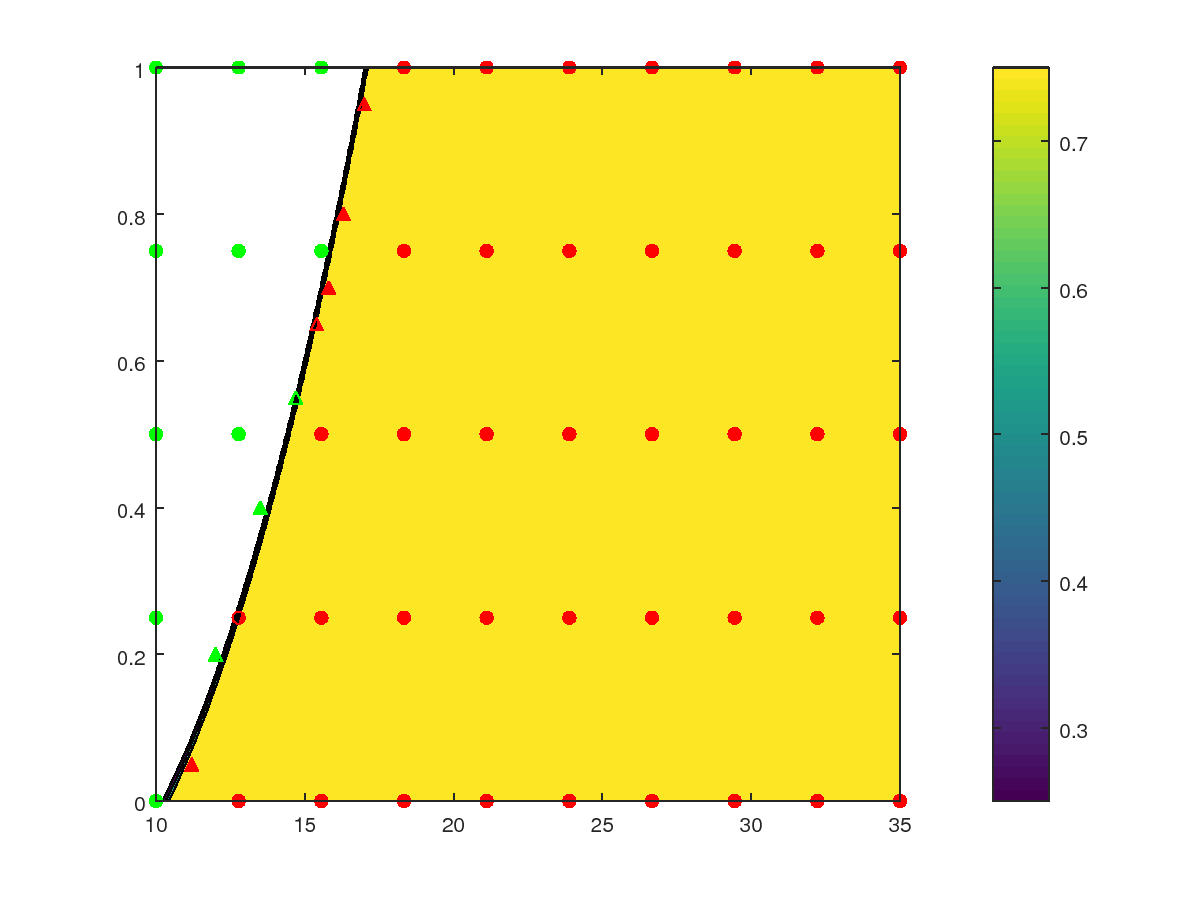
\includegraphics[width=0.75\textwidth]{Figures/classification.png}
  \caption{Binary classification emulator: events reaching $Q_!$ (red) and events not reaching $Q_!$ (green) for $Q_! = XX.X$.}
  \label{fig:classification_Q1}
\end{figure}




\begin{figure}[htpb]
  \centering
  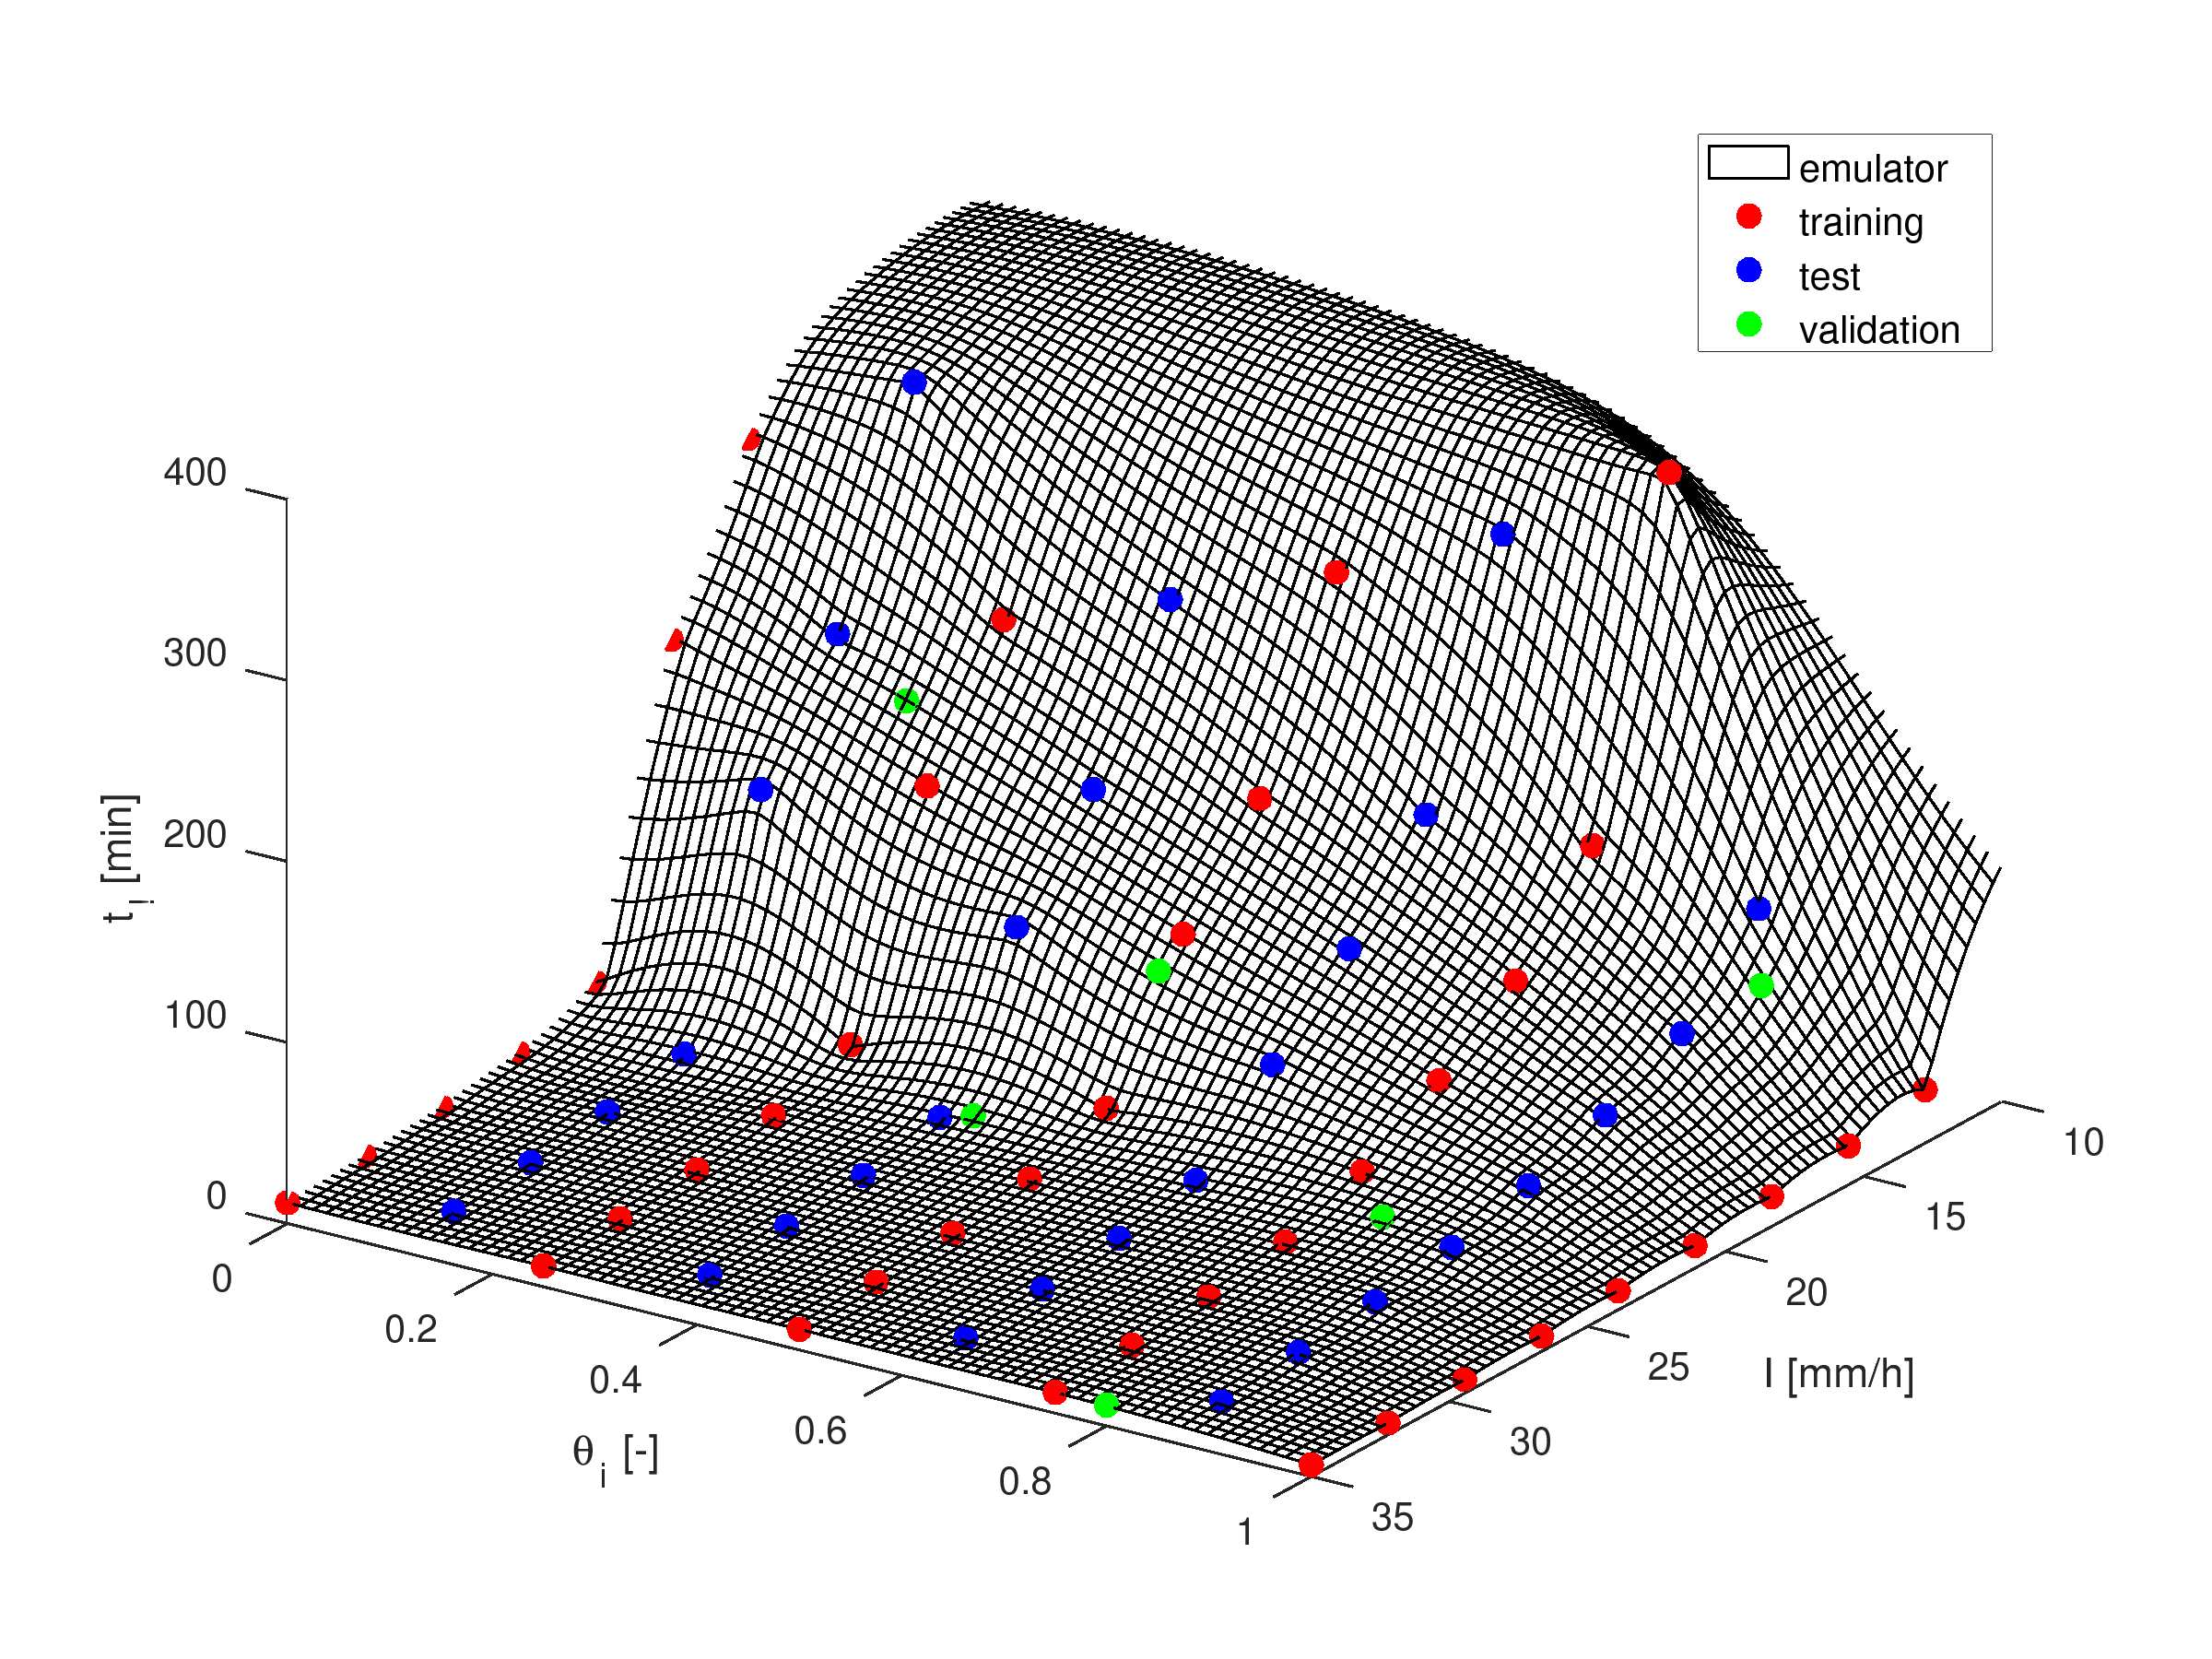
\includegraphics[width=0.7\textwidth]{Figures/emulator.png}
  \caption{Time-to-threshold emulator: training (red), test (blue) and validation (green) datasets and the emulator producing the intrapolation response.}
  \label{fig:}
\end{figure}

% ---------------------------------------------------------------------------------------------------
\subsection{Material and methods}
% ---------------------------------------------------------------------------------------------------

\begin{table}[htpb]
  \centering
  \caption{Emulator performance on \emph{test} and \emph{validation} data}
  \label{table label}
  \begin{tabular}{lcc}
    \toprule
     & \textbf{MAE [\si{\minute}, \si{\percent}]} & \textbf{RMSE [\si{\minute}, \si{\percent}]} \\
    \midrule
    \textbf{test} & val & val \\
    \textbf{validation} & val & val \\
    \bottomrule
  \end{tabular}
\end{table}


% ---------------------------------------------------------------------------------------------------
\subsection{Results and discussion}
% ---------------------------------------------------------------------------------------------------





